\documentclass[14pt]{extarticle}
\usepackage[utf8]{inputenc}
\usepackage{ngerman}
\usepackage{array}
\usepackage{amsmath}
\usepackage{graphicx}
\title{Bericht Todesstern U5 - Transformationen}
\author{Charline Waldrich, Robert Ullmann, Julian Dobrot}
\date{15. Dezember 2015}

\begin{document}

\maketitle
\pagebreak
\tableofcontents

\section{Aufgabenstellung}
Implementierung einer 4x4 Matrix, einer Klasse für Transformationen und einen Szenengraph. Desweiteren soll ein UML Diagramm gezeichnet werden, was den Raytracer nach den Änderungen durch diese Aufgabe wiederspiegelt.
\subsection{UML Diagramm}
Das Klassendiagramm abgeleitet aud der Aufgabenstellung von Übung 5.\\
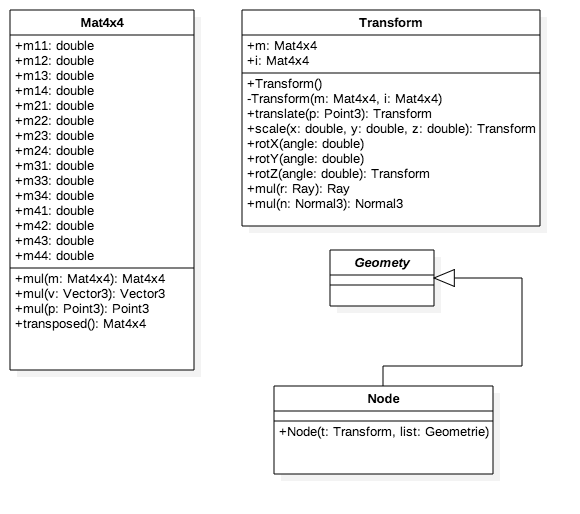
\includegraphics[width=15cm,height=15cm]{images/ClassDiagram}\\

\subsubsection{Anpassungen andere Geometrien}
Nach der Implemntierung des Szenengraphs und dessen Tests können die nun unnötigen Parameter bei den bestehenden Geometrien entfernt werden und können zu folgenden Werten geändert werden:

\begin{itemize} 
\item Beider Kugel für $\vec{c} :=\begin{pmatrix} 0 \\ 0\\ 0 \\\end{pmatrix} $  und für r = 1.
\item Beider Ebene für $\vec{a} :=\begin{pmatrix} 0 \\ 0\\ 0 \\\end{pmatrix} $ und für 
$\vec{n} :=\begin{pmatrix} 0 \\ 1\\ 0 \\\end{pmatrix} $
\item Beider Box für $\vec{a} :=\begin{pmatrix} -0,5\\ -0,5\\ -0,5 \\\end{pmatrix} $ und für
$\vec{b} :=\begin{pmatrix} 0,5 \\ 0,5\\ 0,5 \\\end{pmatrix} $
\end{itemize}

\subsection{Lösungsstrategien}
\subsubsection{UML Diagramm}
Die Klassen Mat4x4, Transform, Node sowie ihre Attribute und Methoden wurden aus dem Aufgabentext übernommen und visualisiert
\subsubsection{Implementierung}
Die Implementierung der Klassen in den Raytracer erfolgte durch die Hinweise aus der Aufgabenstellung, sowie durch die mathematischen Grundlagen zur Transformation aus den Vorlesungen.

\subsubsection{Anpassungen anderer Geometrien}
Nach der Erfolgreichen Implementierung der Klassen mussten noch die nun überflüssigen parameter aus den Geometrien Plane, Sphere und AAB entfernt werden.
\subsubsection{Probleme und besondere Ereignisse}
In der Lösung dieser Aufgabe kam es zu keinen größeren Problemen oder Fehlern. Einzig die anpassung der AAB war etwas aufwendiger. Einige kleinere Fehler in der Mat4x4 konten mit Tests behoben werden.

\subsection{Tests}
Die Abbildung zeigt die Transformierte Kugel aus der Aufgabenstellung.\\\\
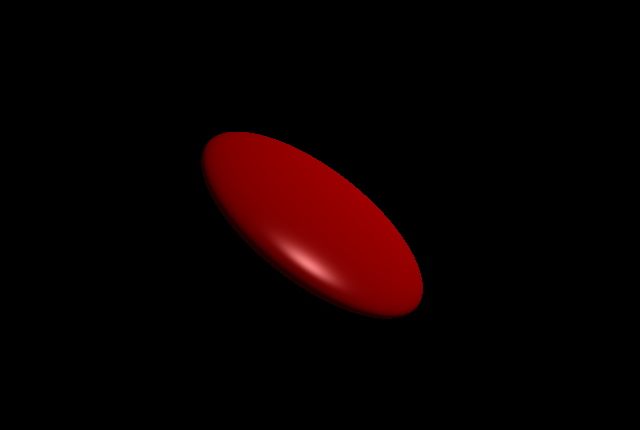
\includegraphics[width=10cm,height=10cm]{images/tr_abb_1}\\\\\\\\\\
Die Abbildung zeigt die Transformierte AAB aus der Aufgabenstellung.\\\\
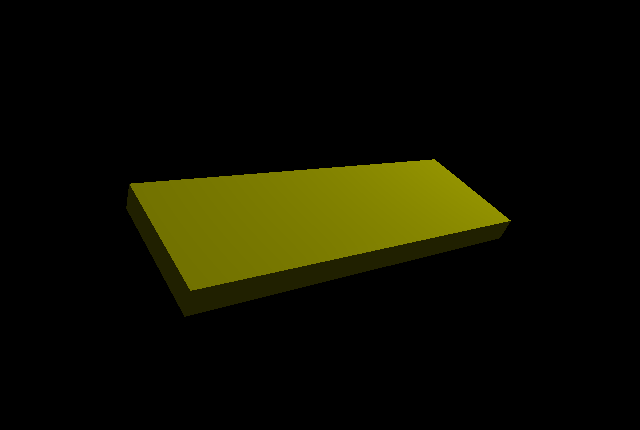
\includegraphics[width=10cm,height=10cm]{images/tr_abb_2}\\

\section{Zeitbedarf}
\begin{center}
\begin{tabular}{cr}
Änderungen an bestehenden Klassen \	&60 min	\\
UML Diagramm	  \	&100 min	\\
Implementiereung 	\	&180 min	\\
Programmierung \	&300 min	\\
Umstellung \	&120 min	\\
Bericht  \		&100 min	 \\
	\hline
	&860 min
\end{tabular}
\end{center}

\section{Quellen}

\end{document}
